\documentclass{mcmthesis}
\mcmsetup{CTeX = false,   % 使用 CTeX 套装时,设置为 true
        tcn =2008722, problem = A,
        sheet = true, titleinsheet = false, keywordsinsheet = true,
        titlepage = false, abstract = true}
\usepackage{newtxtext}%\usepackage{palatino}
\usepackage{geometry}
\geometry{left=1in,right=0.75in,top=1in,bottom=1in}
\usepackage{lipsum}
\title{The \LaTeX{} Template for MCM Version \MCMversion}
\author{\small \href{http://www.latexstudio.net/}
  {
\includegraphics[width=7cm]{mcmthesis-logo}}}
\date{\today}
\usepackage{verbatim}
\begin{document}
\begin{abstract}
Problem 1: carry out kerry gold interpolation on the original data obtained from the Scottish sea area to determine the data in the
research area of our team.The monthly sea surface temperature data from 1980 to 2020 were used to predict the sea surface temperature of each location in the next 50 years in a time series. Finally, the suitable water temperature of herring and mackerel was matched to a specific point, which was the most likely location for mackerel to survive in the next 50 years.The results show:

For problem 2: using the obtained monthly sea surface temperature data of 64 locations from 1980 to 2020, find the locations where most fish species can survive.Then, the maximum monthly catch, the minimum monthly catch and the most likely monthly catch per year from 1980 to 2020 of each position coordinate point were counted. Finally, the moving average method was used to predict the year 2020.Our results are: the maximum time equals 6.925 months;Most likely time equals 4.925 months;The maximum time is equal to 1.270 months;

Aiming at problem 3: the team mainly considered three factors -- cost, profit and the influence of environment on the decision, and then established the decision satisfaction model based on the analytic hierarchy process.Small fishing companies in the northeast Atlantic may not change their practices, and some small fishing companies in the northwest Atlantic may change their practices with option two.

In view of the influencing factors of question 4: the inclusion of foreign fishery policies, the satisfaction of the three schemes of question 3 is adjusted, and the following is obtained:
\begin{keywords}
ARIMA\quad AHP
\end{keywords}
\end{abstract}
\maketitle
%% Generate the Table of Contents, if it's needed.
\thispagestyle{empty}
\tableofcontents

%\newpage
%\thispagestyle{empty}
%\title{fish of scotland}
%\lipsum{5}

%%
%Generate the Memorandum, if it's needed.
%\memoto{\LaTeX{}studio}
%\memofrom{Liam Huang}
%\memosubject{Happy \TeX{}ing!}
%\memodate{\today}
% \logo{\LARGE I'm pretending to be a LOGO!}
%\begin{memo}[Memorandum]
%	\lipsum[1-3]
%\end{memo}

\newpage
\setcounter{page}{1}
%%
\section{Introduction}
\subsection{Background}
Global warming has led to dramatic changes in ocean surface temperatures, which have had a nasty effect on fisheries.Changes in ocean surface temperatures have forced fish to migrate, causing serious losses to countless related industries.Scotland's waters as a world famous fishing area, no doubt has been greatly affected.Our team was invited by the north Atlantic fisheries management association of Scotland to work as consultants to learn more about herring and mackerel in Scotland and to study migration issues around their current habitat in Scotland.
.
\subsection{Restatement of the Problem}%{问题重述}
The following problems will be solved based on the data obtained:

Problem 1: build a model that gives the Scottish north Atlantic fisheries management association some idea of the best migration paths for herring and mackerel around Scotland over the next 50 years, given that water temperatures can change enough to affect herring and mackerel migration.

Problem 2: under the current situation where small fishing companies continue to operate, the model established in question 1 is applied to predict the maximum time, minimum time and most likely time for small fishing companies to catch fish from now on.

Question 3: based on the above forecast analysis, whether small fishing companies should change their way of doing business.Create a model to evaluate the strategy if changes are needed.Two strategies are offered: change company location: move some or all of the company's assets from their current location in a Scottish port to the optimum location from where herring and mackerel migrate.Change the number of fishing boats: use a percentage of small fishing boats to catch fish and keep them fresh.Team other better ideas.

Question 4: what would happen to the proposal for question 3 if the above model were introduced into some fisheries near the territorial waters of other countries?

Question 5: prepare an article or two for Hook Line and Sinker magazine to help fishermen understand the seriousness of the fish migration problem and how proposed solutions can improve the difficulties they face.

\subsection{Overview of Our Work}%{我们做的工作概览}
Problem 1: the Scottish waters are divided into 16 regions, mainly considering the influence of temperature on the migration of two kinds of fish, and ignoring the influence of water quality, predators and food abundance on the migration of fish, the model is simplified to the most, because data is difficult to obtain.Through network query and official website download, the sea surface temperature and corresponding latitude and longitude information in Scottish waters were obtained, and 42×12 months of data were obtained.By using the difference value of kriging method, the 42-year ocean surface temperature data of 16 regions were obtained.A seasonal and periodic time series model was established to predict the ocean surface temperatures in 16 regions over the next 50 years.According to the habits of herring and mackerel to determine the appropriate growth temperature corresponding to the region, this is the best place to live.It must be said that there is more than one optimal location.

Problem 2: understand the maximum, minimum, and most likely time between now and the time it takes for a small fishing company to catch fish as the time interval between the best case, the worst case, and the general case.According to the first model, the best case is defined as the location closest to the small fishery company in the optimal survival location as the fish migration site every time.The worst-case scenario is defined as the best place to live, the farthest from a small fishing company, for every fish migration;The general case is defined as the mean of the best case and the worst case.

Problem 3: if rising sea surface temperatures do affect small businesses' bottom line, help them provide solutions and assess their viability.The evaluation model was established to evaluate the two schemes given and the scheme given by the team.The model mainly considers three factors: cost, fish survival time, and transportation convenience (whether it is suitable for human habitation).

Problem 4: on the basis of question 3, add government factors to adjust the program satisfaction.

Problem 5: combine the conclusions of the first four questions to illustrate our solution for fishermen.

\section{Assumptions and Justifications}
\begin{itemize}
	
	\item It is assumed that there will be no drastic change in sea surface temperature over the next 50 years in English waters;
	
	\item It is assumed that fish demand for living environment in English waters will remain basically unchanged in the next 50 years;
	
	\item It is assumed that the living environment of fish in English waters will not be seriously damaged by external forces in the next 50 years;
	
	\item Fish migration is not considered to be influenced by natural enemies in migratory places, the concentration of chlorophyll in the waters in the migratory areas, and the impact of extreme natural disasters (such as submarine volcanic eruptions in the place where the migration is taking place), the impact of ocean currents on fish survival, and the impact of the amount of food in the place where the migration is taking place.
	
\end{itemize}

\section{Notation}%{符号说明}
\begin{table}[htbp]

	\center
	\begin{tabular}{ccc}
		\toprule
		Symbol & Description \\
		\midrule
		$d$ & the difference order \\
		$p$ & the order of the autoregressive model \\
		$q$ & the order of the moving average \\
		$m$ & the length of the cycle \\
		$\alpha$ & Level is the horizontal smoothing parameter \\
		$\beta$ & Trend is the equilibrium parameter of the trend \\
		$\gamma$ & the smoothing parameter of the season \\
		$x_{t+h}$ & the predicted value for phase h \\
		$T$ & the number of samples (10,000) \\
		$n$ & represents the number of unknown parameters in the model, n=p+q+1 \\
		\bottomrule
	\end{tabular}
	\caption{\label{tab:test}Symbol Description}
\end{table}

\section{Establishment of ARIMA}
\subsection{Model Preparation}
Downloaded from the NOAA website ( http://www.cdc.noaa.gov/ ), the North Atlantic temperature data, the data items include longitude, latitude, depth, temperature. In the data, select data with a depth of 0 and delete the land data. According to the Scottish Marine Fisheries Statistics released by the Scottish Government, from 2016 to 2018 , the top three foreign destinations for fishing boats are Norway, the Republic of Ireland and Denmark. We took this into account when choosing the Scottish fishery range. In the end, the range we selected is shown in the figure, and the longitude and latitude of the data are filtered to obtain the final data. Because not enough data after the screening, and the distribution is not no law, where there is no cause for reference sea surface temperatures, so mining took kriging interpolation of the data extender. It is necessary to pay special attention to the kriging interpolation method for the land surface temperature of our selected area. We were unable to completely delete the terrestrial data, which led to biases in the results below.
The obtained NC format data needs to be processed. Using the Python language NC convert information format required to facilitate processing CSV format, including primary information 1980 in . 1 dated -2019 Year 12 is the month and temperature latitude and longitude, detailed data Appendix.
For the new data obtained, the data that meets the requirements are then screened, that is, the data within the English waters.
\begin{figure}[h]
	\small
	\centering
	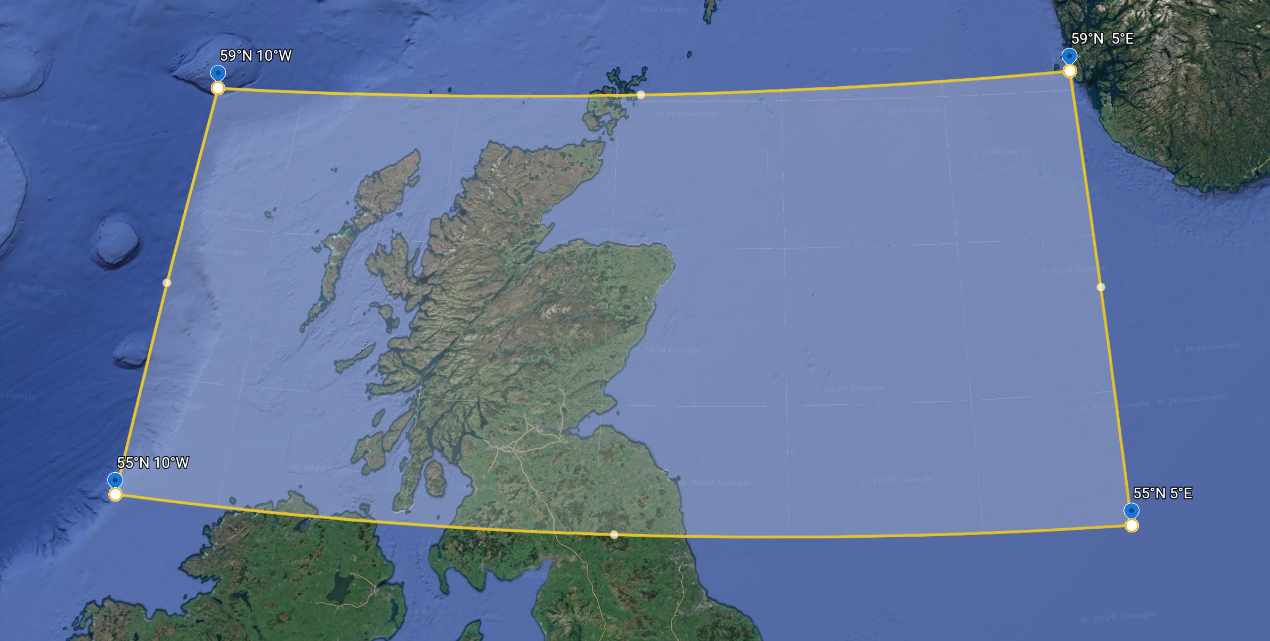
\includegraphics[width=8cm]{question1_p1}
	\caption{Forecast of selected sea area} \label{fig:aa}
\end{figure}

\subsection{Modeling}
1.Identify the stationary of the time series according to the scatter plot, autocorrelation function, and partial autocorrelation function graph.

2. Smooth the non-stationary time series data. Until the value of the autocorrelation function and the processed partial autocorrelation function of the non-significant non- zero.

3. Establish a corresponding time series model based on the identified features. After the smoothing process, if the partial autocorrelation function is censored and the autocorrelation function is tailing, an AR model is established ; if the partial autocorrelation function is tailing and the autocorrelation function is censored , then an AR model is established MA model; if both the partial autocorrelation function and the autocorrelation function are tailing, the sequence is suitable for the ARMA model.

4. Parameter estimation to test whether it has statistical significance.

5. Hypothesis test to determine whether the (diagnostic) residual sequence is a white noise sequence.

6. Make predictions using the tested model.

The ARIMA ( p , d , q ) model can be expressed as:

\[
\left(1-\sum_{i=1}^{p} \phi_{i} L^{i}\right)(1-L)^{d} X_{t}=\left(1+\sum_{i=1}^{q} \theta_{i} L^{i}\right) \varepsilon_{t}
\]

L is a lag operator, representing several periods of lag. It can be understood as a time factor, because this is a model of time series predictive analysis; it is an autocorrelation coefficient, the degree of influence of one thing in different periods; it is a partial correlation coefficient, in multi-element events, and other events are considered as constants. the relevant amount;

d is the difference order;

p is the order of the autoregressive model;

q is the order of the moving average.

Using SPSS uses temperature solving software Laid addition model, which is suitable for containing the data type linear trend and season stabilizing component.

\[
\left\{\begin{array}{l}
{l_{t}=\alpha\left(x_{t}-s_{t-m}\right)+(1-\alpha)\left(l_{t-1}+b_{t-1}\right)} \\
{b_{t}=\beta\left(l_{t}-l_{t-1}\right)+(1-\beta) b_{t-1}} \\
{s_{t}=\gamma\left(x_{t}-l_{t-1}-b_{t-1}\right)+(1-\gamma) s_{t-m}} \\
{\hat{x}_{t+h}=l_{t}+h b_{t}+s_{t+h-m(k+1)}, k=\left[\frac{h-1}{m}\right]}
\end{array}\right.
\]

m is the period length, monthly data is 12 and quarterly data is 4;

α is the horizontal smoothing parameter

β is the trend's balance parameter is the seasonal smoothing parameter

\(\gamma\) is the smoothing parameter of the season

\(x_{i+h}\) is the predicted value for period h

Partial autocorrelation function:

\(\rho_{X_{i}, X_{i+k} | X_{i-1}, \cdots, X_{t+1}}=\frac{E\left[\left(X_{t}-\hat{E} X_{t}\right)\left(X_{t-k}-\hat{E} X_{t-k}\right)\right]}{E\left[\left(X_{t-k}-\hat{E} X_{t-k}\right)^{2}\right.}\)
\(\hat{E} X_{t}=E\left[X_{t} | X_{t-1}, \cdots, X_{t-k+1}\right], \hat{E} X_{t-k}=E\left[X_{t-k} | X_{t-1}, \cdots, X_{t-k+1}\right]\)

The Q test tests whether the residuals are white noise:

\(H_{0}: \rho_{1}=\rho_{2}=\cdots=\rho_{s}=0, H_{1}: \rho_{i}(i=1,2, \cdots, s)\)At least one is not 0

Under the condition that \(H_{0}\) holds, the statistic

\[
Q=T(T+2) \sum_{k=1}^{s} \frac{r_{k}^{2}}{T-k} \sim \chi_{s-n}^{2}
\]

The software will calculate the p- value for us . If the p- value is less than 0.05 , the null hypothesis is rejected. At this time, the model is not fully identified and needs to be modified.

T represents the number of samples

n is the number of unknown parameters in the model, n = p + q + 1

\subsection{stationarity test}
Test position corresponding to the latitude and longitude of each 1980 years . 1 January to 2019 years 12 is dated were 480 ocean surface temperature data samples months timing chart, determining whether the sequence value is always fluctuate around a constant, and fluctuation scope To determine whether the data series are stationary. If not, then the data sequence is a non- stationary sequence, and a difference operation is required to make the sequence a stationary sequence.

\begin{figure}[h]
	\small
	\centering
	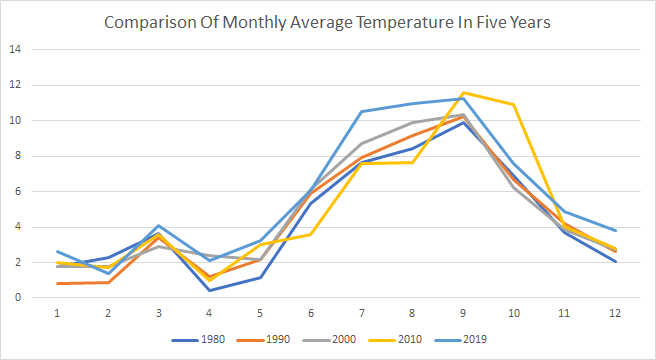
\includegraphics[width=8cm]{temp_fore_tendency_p2}
	\caption{Temperature prediction trend} \label{fig:aa}
\end{figure}

The picture above is the trend chart of the sea coordinate points (58.5N , 185E) closer to the port in 1980 , 1990 , 2000 , 2010 , and 2019. It can be seen that the surface temperature of the ocean is indeed at 10-year intervals. The increase is consistent with the recognition of this question. It can be seen from the time series diagrams of the ocean surface temperature corresponding to multiple latitudes and longitudes in the appendix that the ocean surface temperature corresponding to the latitudes and longitudes at the sea position may be stable or not. Below we select two representative maritime coordinate points to analyze them. The coordinate point (58.5N , 185E) is near the port point, and the temperature will change greatly due to human activities. The coordinate point (55.5N , 170W) is a point at the far port and near the center of the sea, and human activities have a small effect on its temperature .

\begin{figure}[h]
	\small
	\centering
	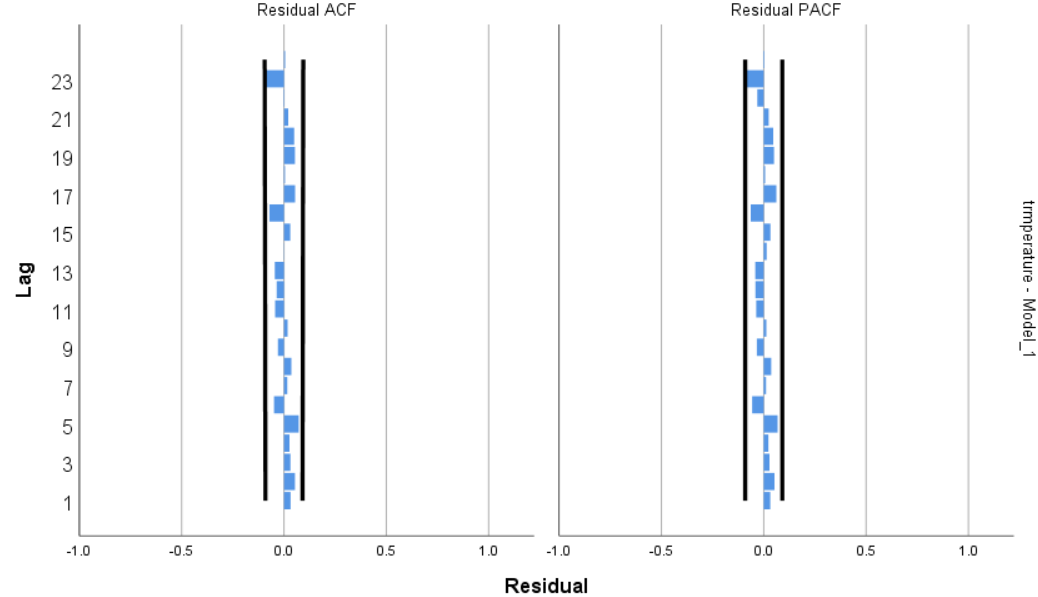
\includegraphics[width=8cm]{question1_p3}
	 \label{fig:aa}
\end{figure}

\begin{figure}[h]
	\small
	\centering
	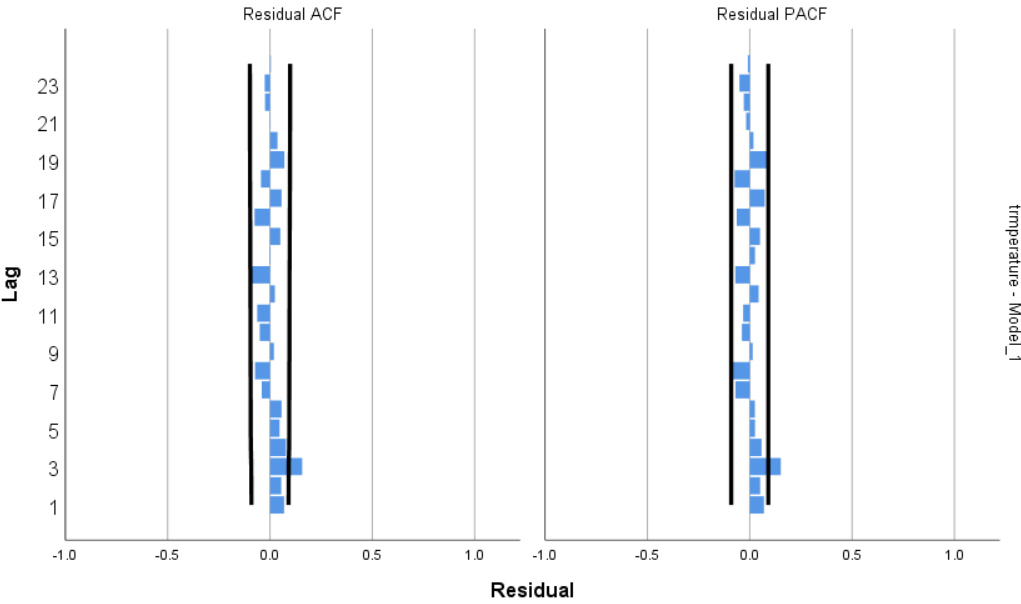
\includegraphics[width=8cm]{question1_p4}
	\label{fig:aa}
\end{figure}

The picture on the left is the autocorrelation diagram and partial autocorrelation diagram of (58.5N , 185E) . Their autocorrelation function and partial autocorrelation function both fluctuate around 0 , so they are stable, but they do not trend after a certain order At 0 , so all are tailing. The picture on the right is the autocorrelation diagram and partial autocorrelation diagram of (55.5N , 170W) . Their autocorrelation function and partial autocorrelation function both fluctuate around 0 , so they have stability. However, none of them apparently tend to 0 after a certain order , so they are all tailing. According to the SPSS automatic generation model, p, d, q in the model can be obtained . 

\subsection{Pure Randomness Test}
Pure random testing, also known as white noise test, the corresponding position by 1980 Nian 1 January to 2019 Nian 12 Yue A total of 480 months of ocean surface temperature data samples were obtained from the autocorrelation coefficients of each delay period, and the test statistics were calculated. When Sig.1 = 0.345> 0.05 , the sequence 2 is indeed a white noise sequence; when Sig.2 = 0.000 <0.05 , the sequence 1 has autocorrelation, and it is not all white noise. The stable R- squared 1 = 0.683 and the stable R- squared 2 = 0.696 , so the model's prediction ability is better. 
\subsection{Predicting temperatures for the next 50 years at various points}
\begin{figure}[h]
	\small
	\centering
	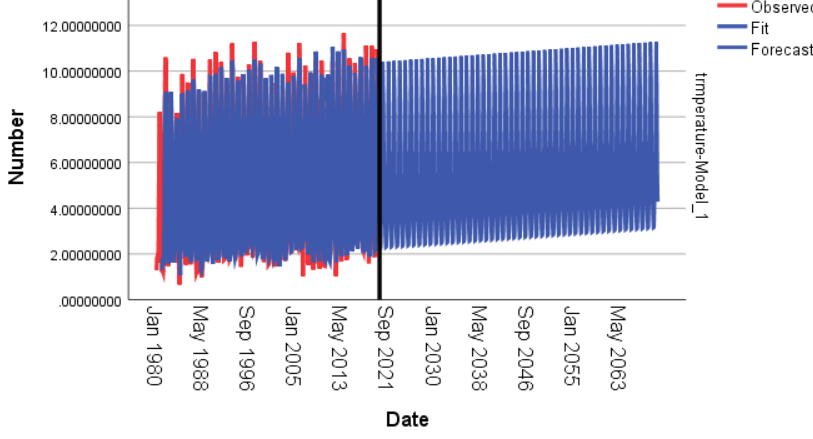
\includegraphics[width=8cm]{question1_p5}
	\label{fig:aa}
\end{figure}

\begin{figure}[h]
	\small
	\centering
	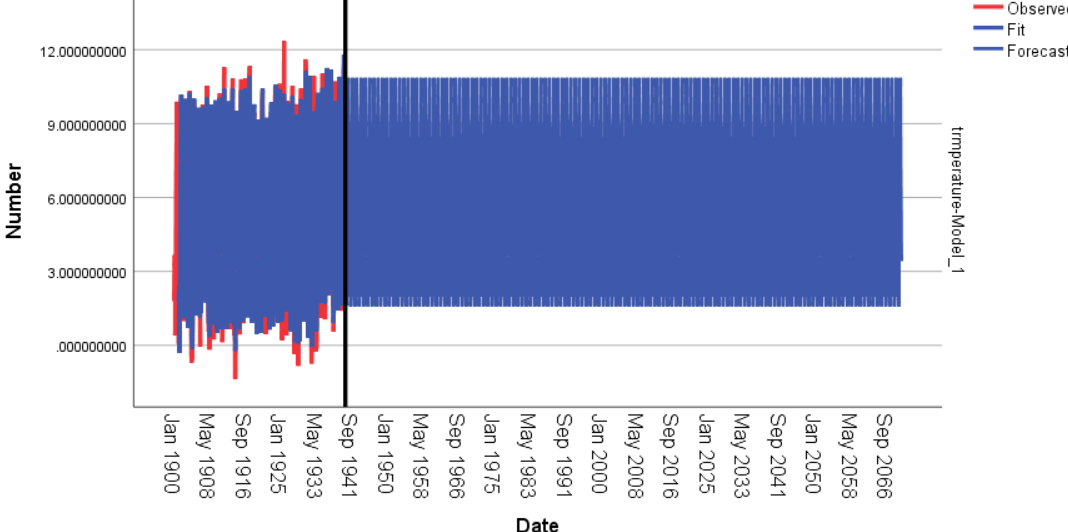
\includegraphics[width=8cm]{question1_p6}
	\label{fig:aa}
\end{figure}

At left (58.5N , 185E) on the next 50 years the monthly forecast sea surface temperature, we can clearly see that the temperature is on the rise; right picture (55.5N , 170W) on the future of 50 years each The prediction of the monthly ocean surface temperature can clearly be seen as a relatively stable temperature within a range without a significant upward trend.

\subsection{Predicted Location}
Based on the data obtained has been checked: Water temperature herring suitable for survival is 3 to 6 degrees Celsius, mackerel fish 6-7 water temperature in February is suitable for survival of 6 to 10 degrees Celsius. The water temperature here refers to the ocean surface temperature. Based on the predicted ocean surface temperatures for each of the coordinates in the next 50 years, plus the appropriate ocean surface temperatures of the two fishes, a suitable location for herring and mackerel for each month in the next 50 years is obtained. Only part of the prediction results are given below.
\begin{figure}[h]
	\small
	\centering
	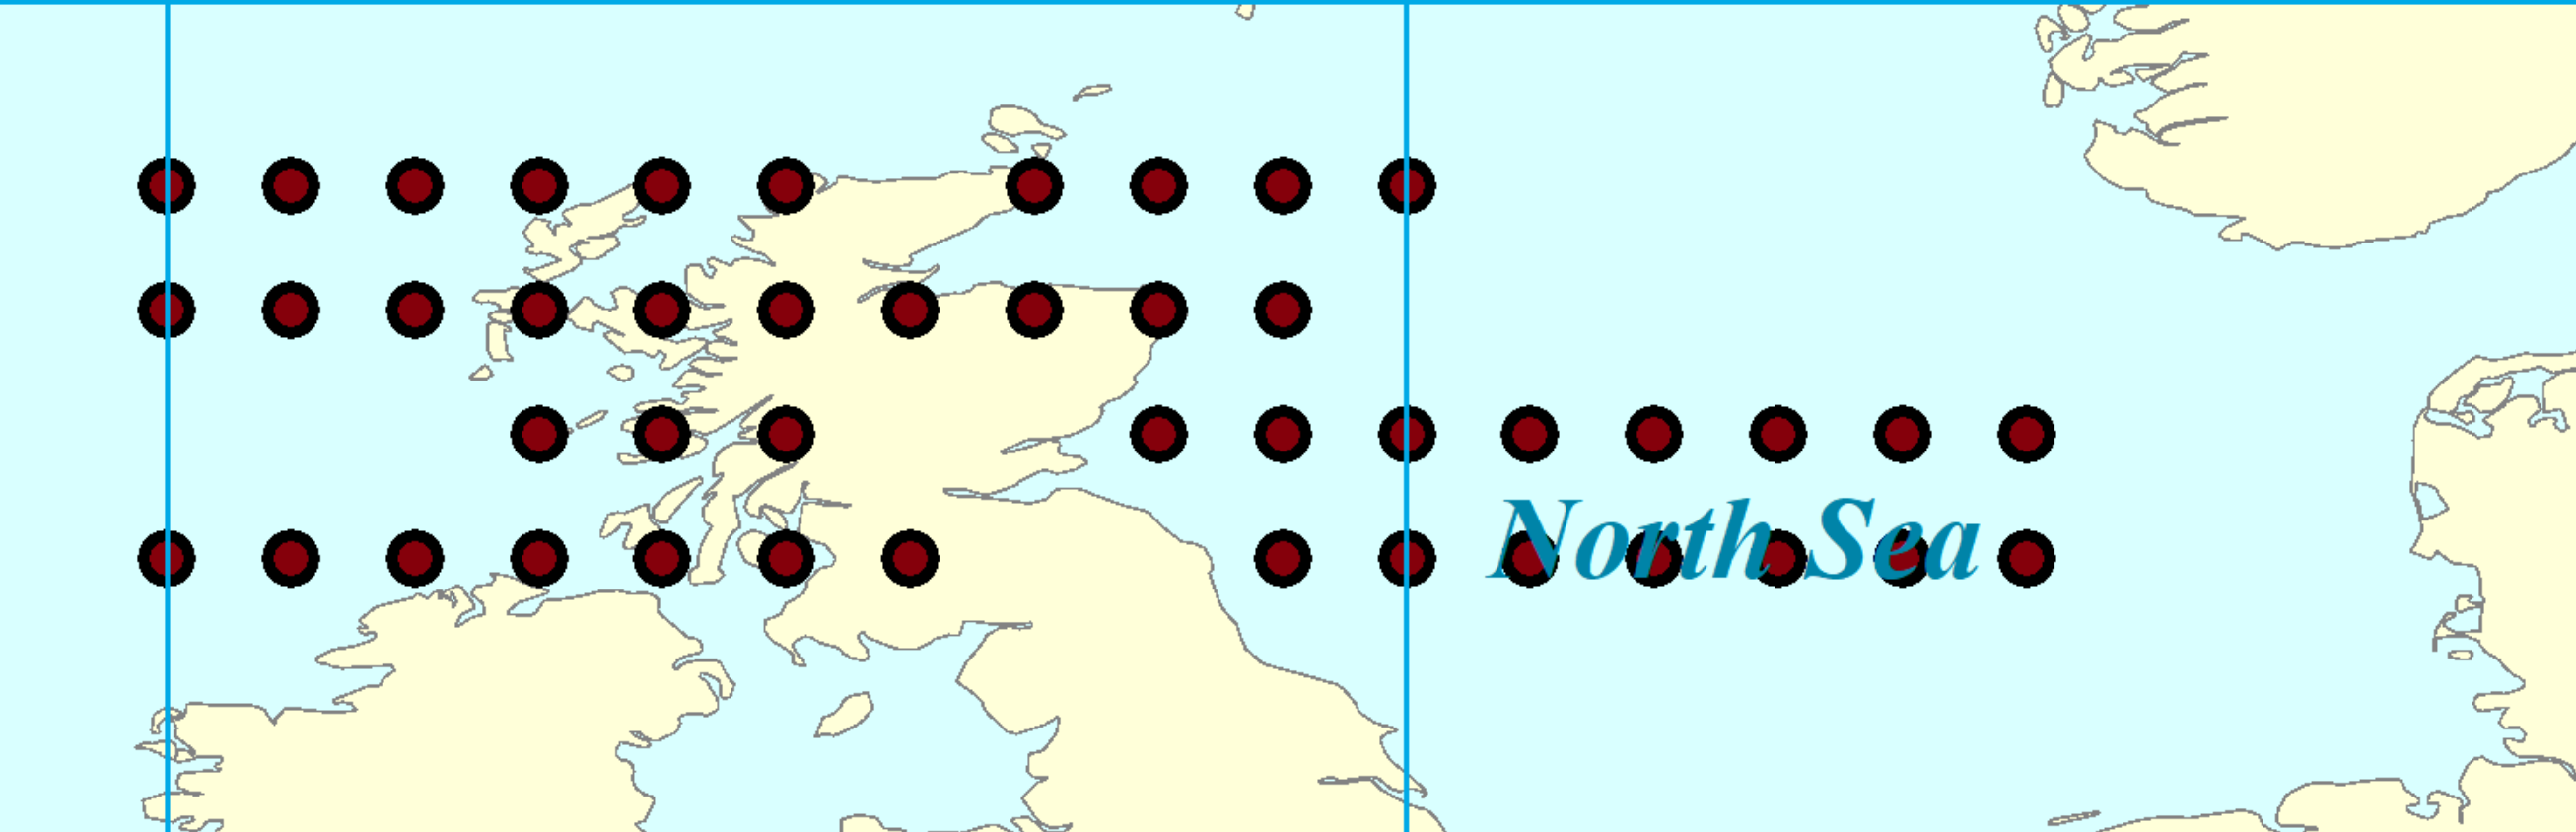
\includegraphics[width=8cm]{h206901}
	\caption{Most likely herring to survive in January 2069} \label{fig:aa}
\end{figure}

We can see that some points in the above picture are unreasonable. For example, they are on land. This is caused by insufficient data cleaning and cannot be avoided. The above two can be seen in FIG 2069 years . 1 month, and 2069 years . 4 dated Herring most likely position is substantially the same as described herring possible stay time portion of this area is very long. The water temperature has a certain effect on its migration. We found that if the points on the land can be deleted, then the position in the northwestern Atlantic is less than that in the northwestern Atlantic, which is consistent with the actual distribution of herring population.

\begin{figure}[h]
	\small
	\centering
	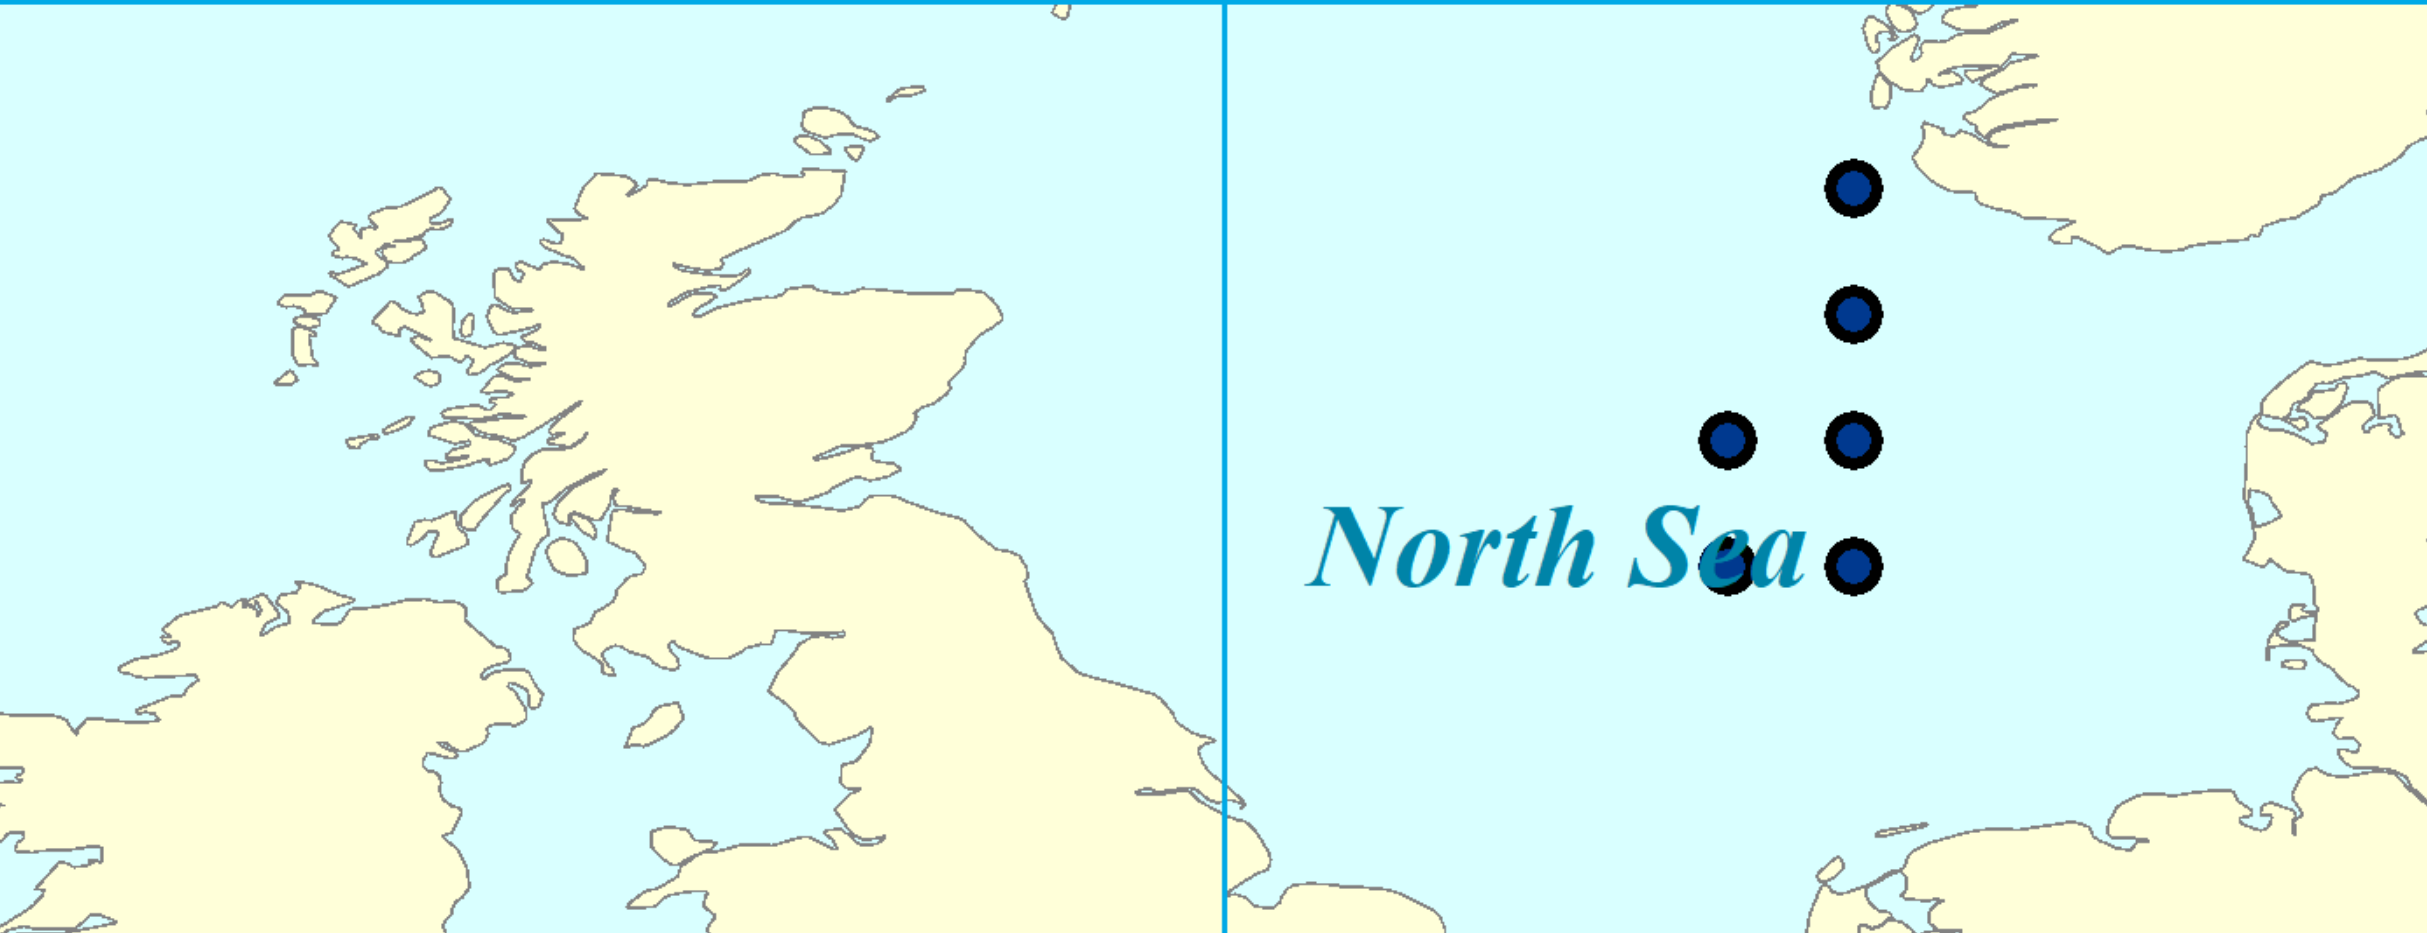
\includegraphics[width=8cm]{h19801}
	\caption{The most likely locations for herring to survive in January 1980} \label{fig:aa}
\end{figure}

Comparing the above picture with the most likely location for herring in January 2069, we can clearly see that the number of locations suitable for herring survival has increased. As the surface temperature of the ocean increases, herrings increasingly prefer the temperature of the North Atlantic because the temperature here is more suitable for them. This supports the fact that thermal preferences can be subordinated to reproductive needs.

\begin{figure}[h]
	\small
	\centering
	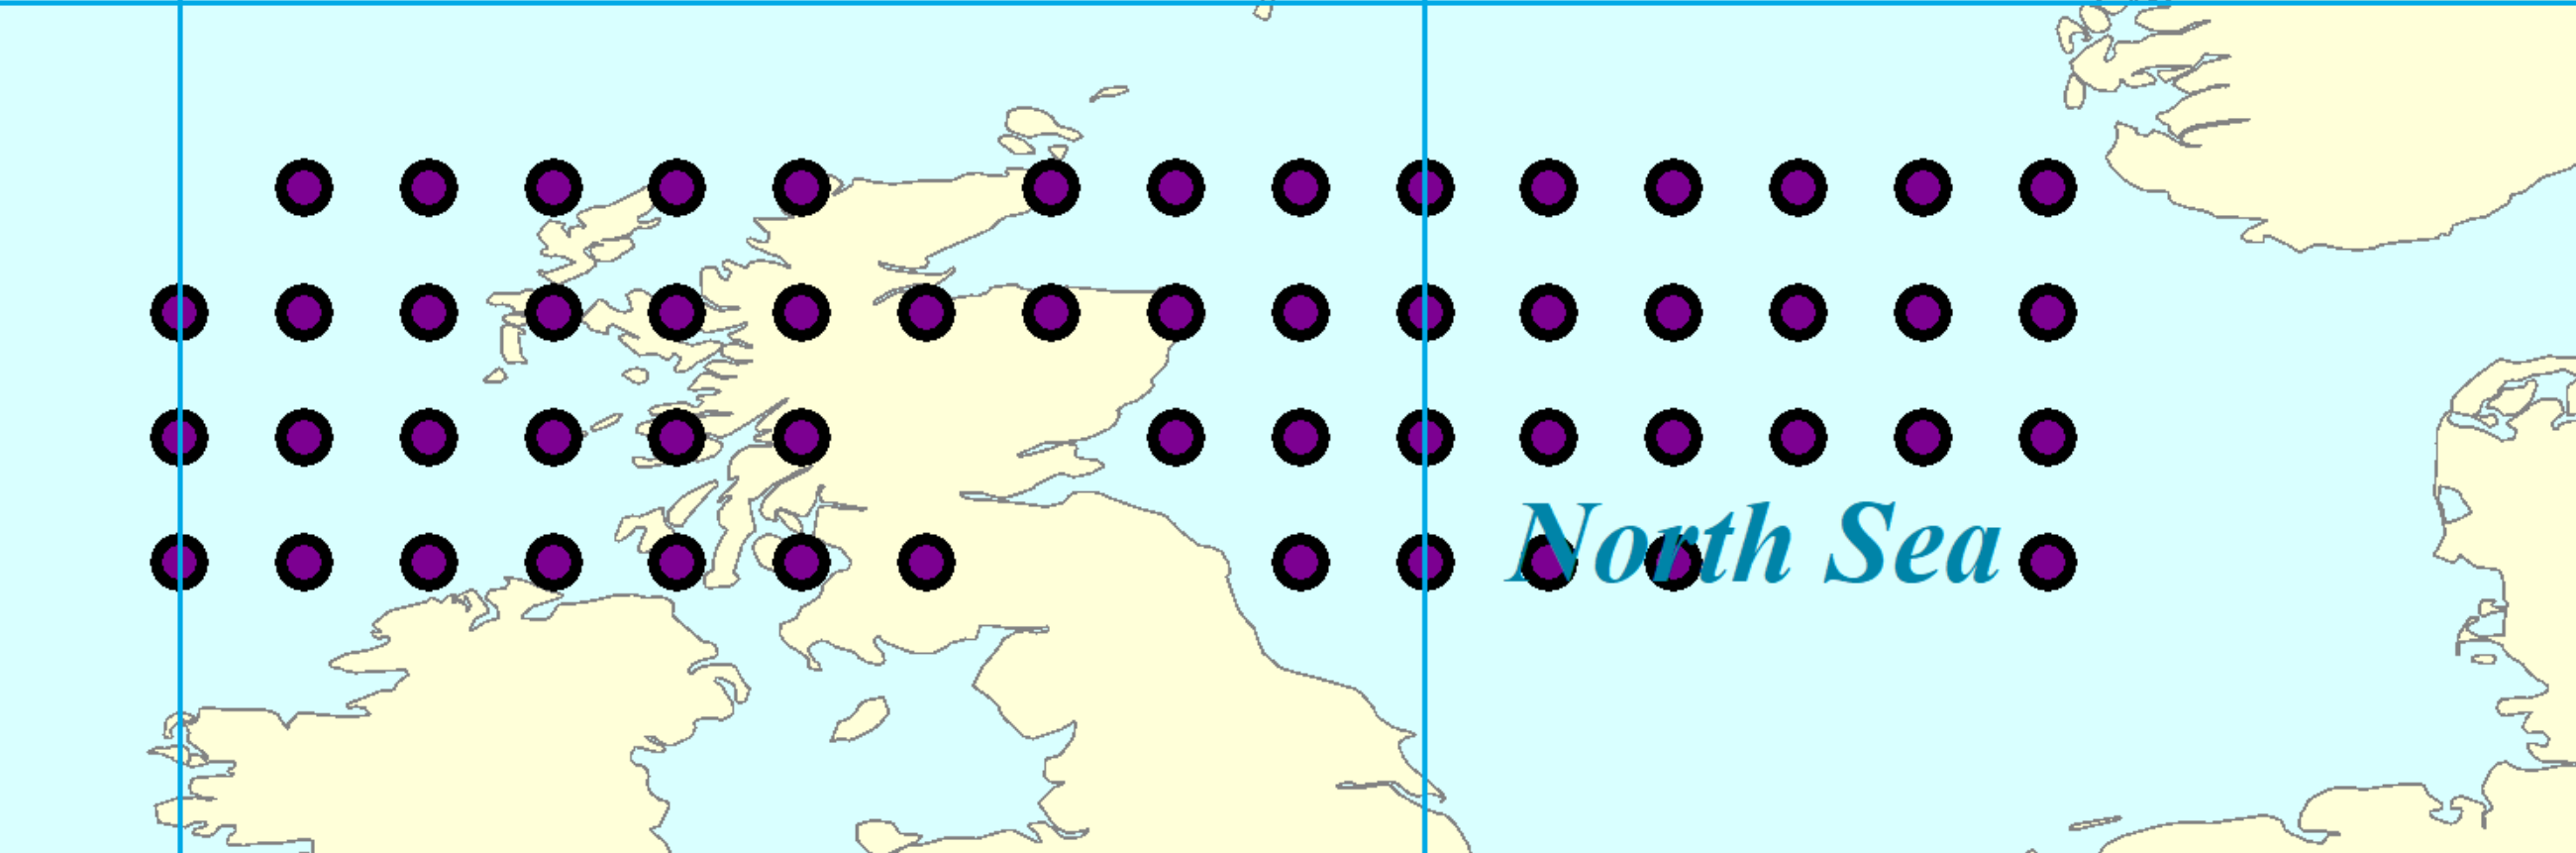
\includegraphics[width=8cm]{m206907}
	\caption{Where mackerel is most likely to survive in July 2069} \label{fig:aa}
\end{figure}

\begin{figure}[h]
	\small
	\centering
	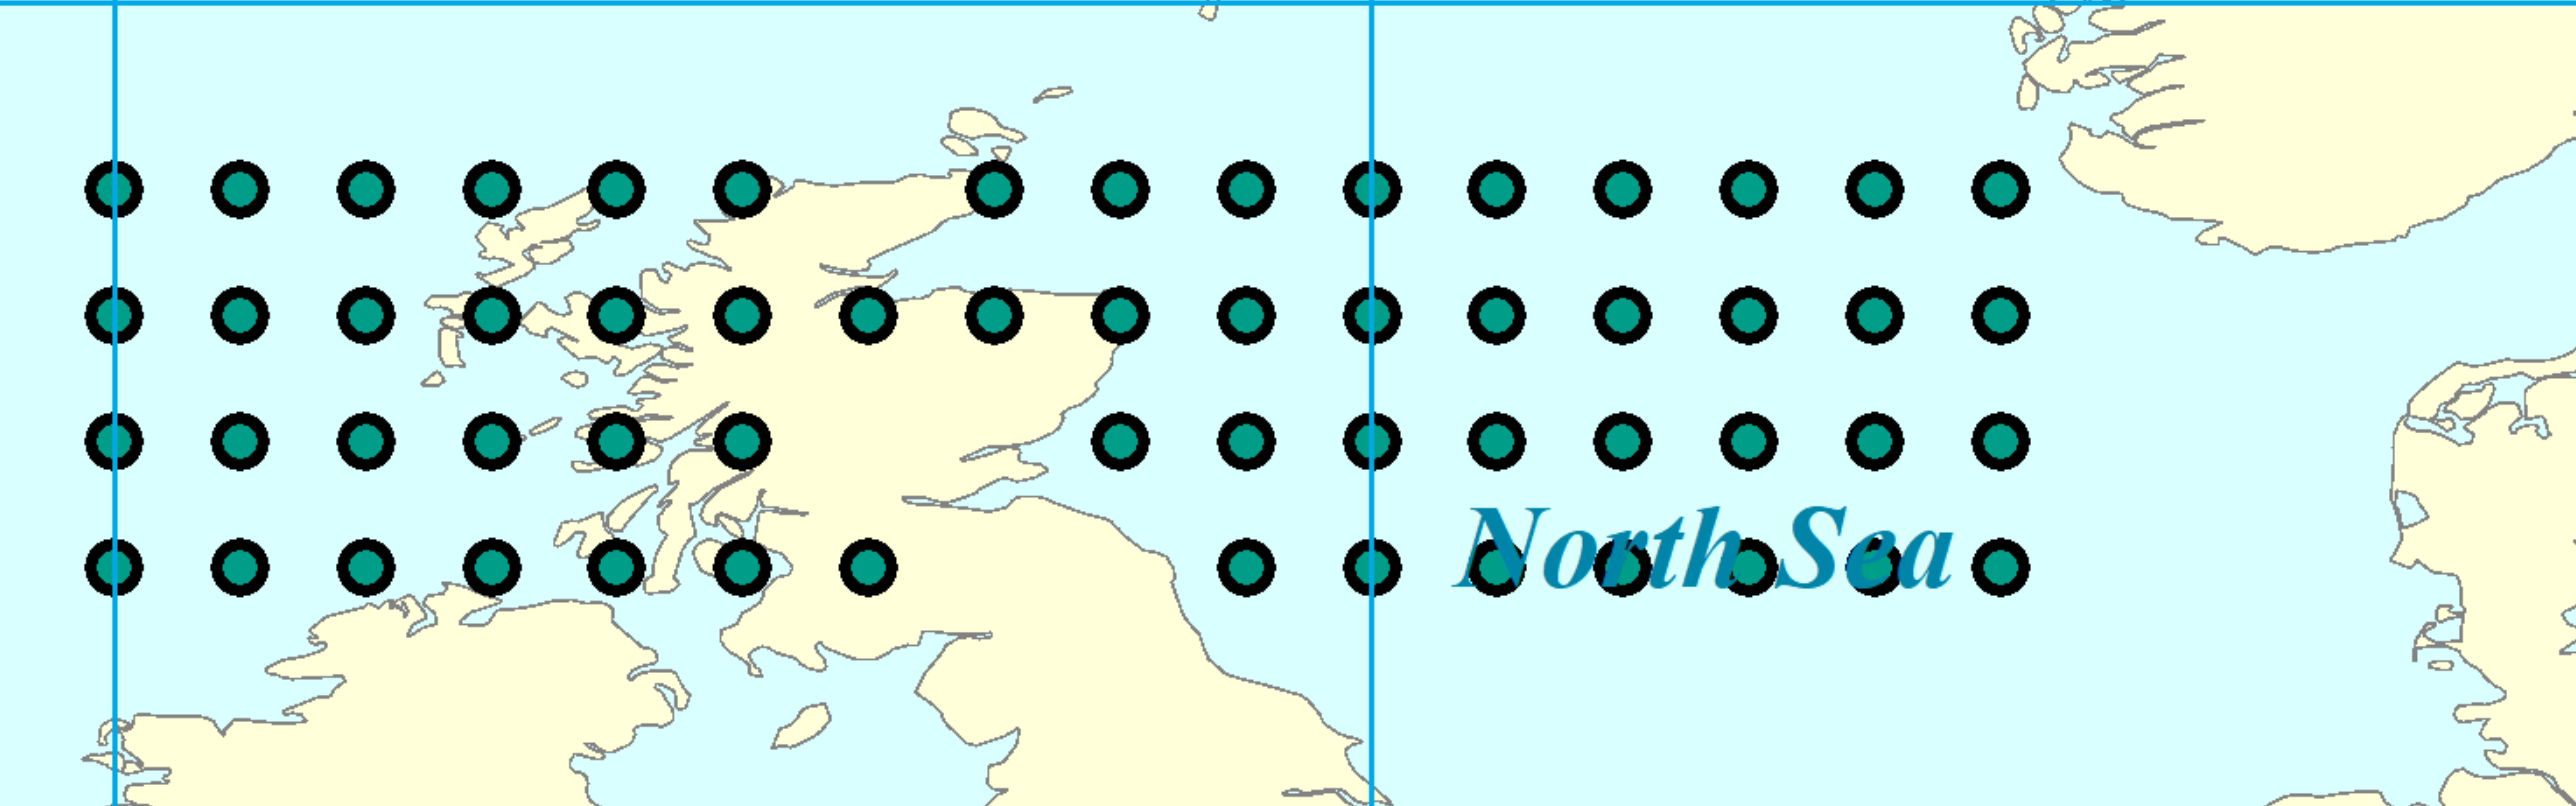
\includegraphics[width=8cm]{m206910}
	\caption{The most likely place for mackerel to survive in October 2069} \label{fig:aa}
\end{figure}

The two pictures above show that the most likely locations for herring in January 2069 and April 2069 are roughly the same, indicating that mackerel may stay in this area for a long time. The water temperature has a certain effect on its migration.

\section{analytic hierarchy process}
\subsection{Model Introduction}
Modeling with analytic hierarchy process can be roughly performed in the following four steps:

( I )\quad establishing a hierarchical structure model;

( II )\quad constructing all judgment matrices in each level;

( III ) hierarchical ranking and consistency check;

( IV )  Hierarchical total ordering and consistency check.

We consider the impact of three factors: cost, profit, and environment on decision making. Then the importance of the three factors is obtained by constructing the judgment matrix.Then we have to check whether the construction matrix is correct and whether it meets the consistency. When the consistency test is satisfied, the judgment matrix is correct and there is no big logical contradiction.

\begin{figure}[!htp]
	\centering
	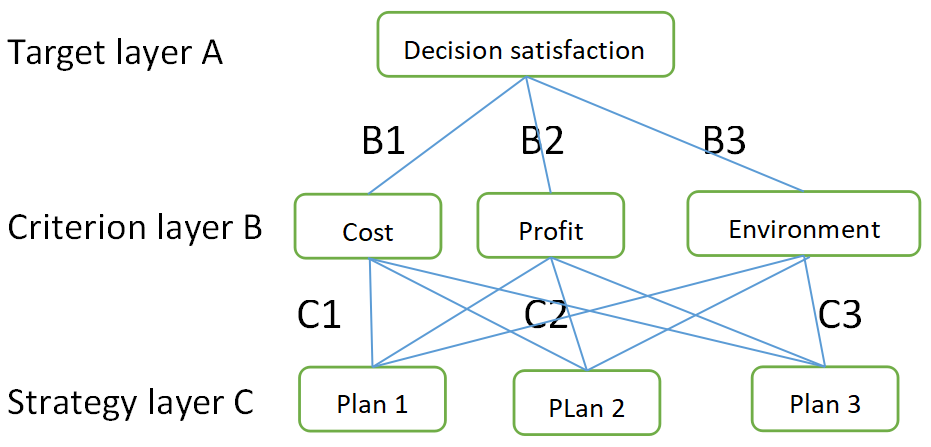
\includegraphics[width=8cm]{layer_p.png}\\
	\caption{Hierarchical model}
\end{figure}

Construct a judgment matrix:
\begin{equation}
A=\left[\begin{array}{cccc}
{\frac{w_{1}}{w_{1}}} & {\frac{w_{1}}{w_{2}}} & {\cdots} & {\frac{w_{1}}{w_{n}}} \\
{\frac{w_{2}}{w_{1}}} & {\frac{w_{2}}{w_{2}}} & {\cdots} & {\frac{w_{2}}{w_{n}}} \\
\cdots &\cdots &\cdots  &\cdots\\
{\frac{w_{n}}{w_{1}}} & {\frac{w_{n}}{w_{2}}} & {\cdots} & {\frac{w_{n}}{w_{n}}} \\
\end{array}\right]
\end{equation}

Consistency ratio CR :
\begin{equation}
C R=\frac{C I}{R I}
\end{equation}
Among them:

$R I=\frac{\lambda_{\max }^{\prime}-n}{n-1}$,$C I=\frac{\lambda_{\max }-n}{n-1}$

$\lambda_{\max }$ is the maximum eigenvalue of matrix A ;

$\lambda_{\max }^{'}$ is the average of the largest characteristic roots;

n is the order of the matrix A.

When$ CR < 0.10 $, it is considered that the consistency of the judgment matrix is acceptable, otherwise the judgment matrix should be modified appropriately.

\subsection{Model preparation}
\begin{figure}[!htp]
	\centering
	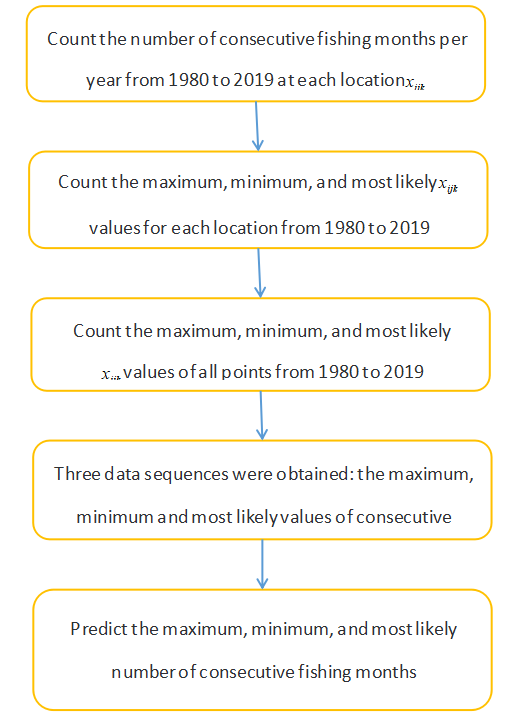
\includegraphics[width=8cm]{question2_p1.png}\\
	\caption{Hierarchical model}
\end{figure}
Considering the suitable water temperature for two types of fish, a surface temperature of 3-10 degrees Celsius can make at least one of the two types of fish survive. We will now small-scale fishing companies catch any fish the longest time, the shortest time, and the most likely time to be understood as the best case, worst case, and when in the general case interval. Here we assume that small-scale fisheries companies only fish at a certain location due to their small size. We will replace the long-term fishing time of small-scale fisheries companies in one place with the number of months that a certain location can continuously fish. Because we have data for the past forty years, we can get the number of months that can be continuously fished each year at each point in the forty years. The calculation method is as follows:

1. Number of months of continuous fishing each year at each location

$x_{i j k}=$ The number of months that satisfy this condition $\quad \mathrm{i}=1-40, \mathrm{j}=1-64,0 \leq \mathrm{k} \leq 6$

2. All positions 1980-2019 per year between the years of maximum, minimum, and most likely value:

$x_{i}^{1}=\max x_{i j k}$ represents 1980-2019 the number of months the maximum annual fishing consecutive sequence;

$x^{2}_{i}=\operatorname{avg} x_{i j k}$ pepresents the most probable value sequence representing the number of months of continuous fishing each year from 1980 to 2019;

$x^{3}_{i}=\min x_{i j k}$ represents 1980-2019 the number of months the minimum sequence of consecutive annual fishing

According to the ARIMA model for prediction, it is found from the prediction results that the ARIMA model is not suitable, so it is better to take a moving average score. The following is our result.

\begin{figure}[!htp]
	\centering
	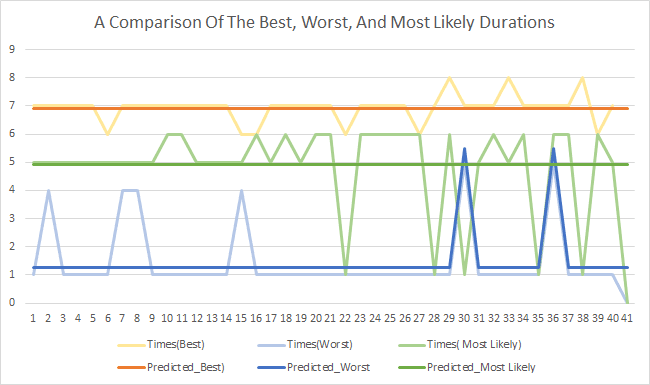
\includegraphics[width=8cm]{question2_p2.png}\\
\end{figure}

As can be seen from the above figure, the fishing situation in each region varies greatly each year and it is difficult to predict. Our results are: the maximum time is equal to 6.925 months; the most likely time is equal to 4.925 months; the maximum time is equal to 1.270 months; this is consistent with the peak fishing season.

\subsection{Model establishment}

\begin{figure}[!htp]
	\centering
	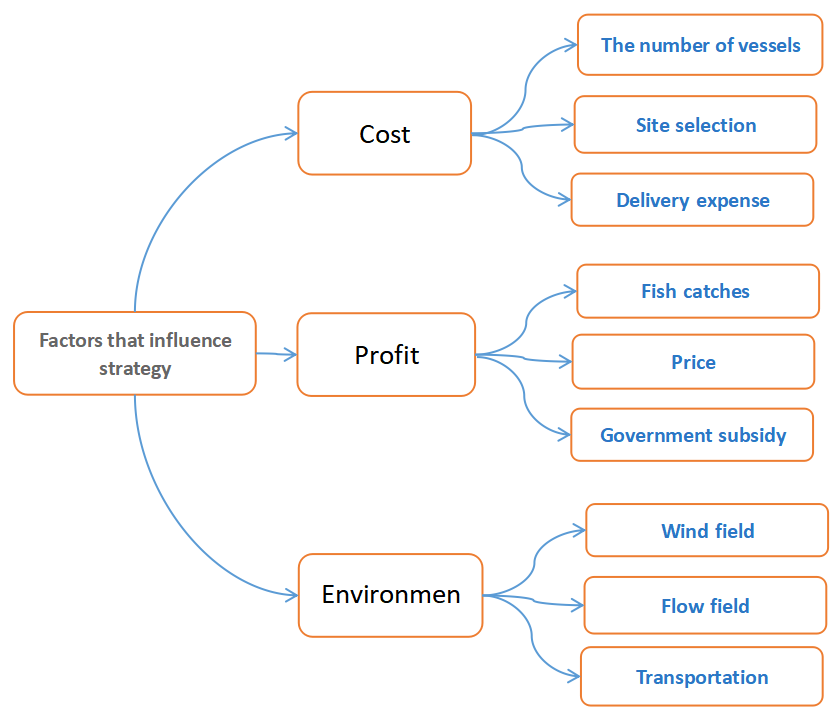
\includegraphics[width=8cm]{question_p1.png}\\
	\caption{Correlation diagram of factors considered by AHP}
\end{figure}

Consider the impact of three broad areas on strategy choices: cost, profit, and environment. Cost is mainly affected by the number of fishing boats purchased, relocation options and transportation costs; profits are mainly affected by fishing volume, fish price fluctuations and government subsidy policies. Environmental factors mainly consider the influence of wind field, flow field and transportation convenience.

Three options are being considered.

Option 1 : Change the location of the company: Transfer some or all of the company's assets from their current location in Scottish ports to the best location away from where herring and mackerel migrate.

Option 2 : Change the number of fishing boats: Use a small percentage of small fishing boats to catch fish and ensure the freshness of the fish.

Option 3 : Change the company's location and increase the number of fishing vessels.

Firstly, three factors in the criterion layer are compared in pairs according to the importance, and the judgment matrix is obtained.

\begin{figure}[!htp]
	\centering
	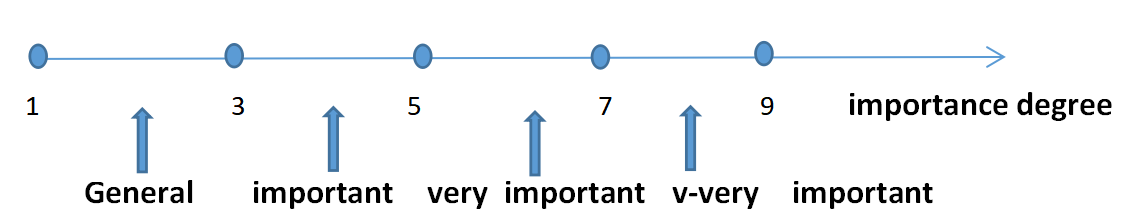
\includegraphics[width=8cm]{question3_p2.png}\\
	\caption{Meaning of scale}
\end{figure}

The judgment matrix A is obtained from the meaning of the coordinates , and other judgment matrices are obtained by the same method.

\[
\begin{pmatrix}{*{20}c}
{a_{11} } & {a_{12} } & {a_{13} }  \\
{a_{21} } & {a_{22} } & {a_{23} }  \\
{a_{31} } & {a_{32} } & {a_{33} }  \\
\end{pmatrix}
\]

$
A=\left[\begin{array}{ccc}
{1 / 1} & {3 / 9} & {3 / 5}  \\
{9 / 3} & {1 / 1} & {9 / 5}  \\
{5 / 3} & {5 / 9} & {1 / 1}  
\end{array}\right]
$

The CRs of the four judgment matrices are 0.0000 , 0.0032 , -0.0000 , and 0 are all less than 0.10 , and the consistency check is acceptable. Finally, the result of analytic hierarchy process is obtained. Option 1 scored 0.2784 , Option 2 scored 0.4217 , and Option 2 scored 0.2999 . It can be seen from the results that the second scheme is better. If small fisheries companies are to change their economic strategies, they should give priority to the second option. Our team based on the results of the first two models: Because the migration of mackerel and herring changes northward due to temperature, small fisheries companies in the northeast Atlantic can not change their operating methods, and some small fisheries in the northwest of the Atlantic Fisheries companies can adopt the second option to change the way of business.

\subsection{Optimization of fishery model after migration}
According to the traditional law of the sea , the territorial sea is the high seas ; the territorial sea is under the sovereignty of the coastal states , but restricted by the innocent passage of foreign ships ; the high seas are open to all countries and the high seas are free. In terms of fishing , coastal States enjoy exclusive fishing rights in territorial waters , no other country has the right to fish in the territorial sea of the coastal State; coastal States the right to prohibit or restrict foreign to engage in fishing activities within its territorial sea , and the coast Fishing rights are fully reserved for nationals. With the approval of a coastal State or another agreement between the two countries or on the basis of reciprocity , the coastal State usually allows foreign countries to fish in its territorial sea. 

Britain in Europe before de EU's Common Fisheries Policy in Scotland if you want to fishermen fishing in other EU countries, Britain off Europe must re-negotiate individual countries and fisheries policy after.

Assume that after some time the British and other countries have negotiated fisheries. Fishing vessels can be harvested in countries where some fisheries are transferred, but companies cannot be relocated to that country. Therefore, the hierarchical structure of the analytic hierarchy process model used in the previous question adds the factors of fishery transfer on the criterion level.

The first step is to build a new hierarchy diagram

\begin{figure}[!htp]
	\centering
	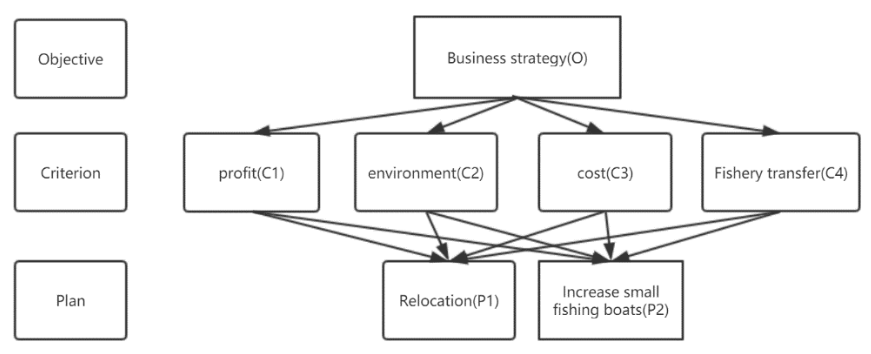
\includegraphics[width=8cm]{question4_p1.png}\\
	\caption{Meaning of scale}
\end{figure}

The second step is to build a judgment matrix
$$Judgment matrix O-C$$
$$
\begin{array}{|c|c|c|c|c|}
\hline  & {{Cl}} & {{C} 2} & {{C} 3} & {{C} 4} \\
\hline {Cl} & {1} & {2} & {4} & {8} \\
\hline {C2} & {0.5} & {1} & {2} & {4} \\
\hline {C3} & {0.25} & {0.5} & {1} & {2} \\
\hline {C4} & {0.125} & {0.25} & {0.5} & {1} \\
\hline
\end{array}
$$


The third step uses the judgment matrix to calculate the relative weight of the compared elements to the criterion by using the arithmetic average method, geometric average method, and eigenvalue method.
$$Weight matrix O-C$$
$$
\begin{array}{|c|c|c|c|}
\hline C & {\text { Arithmetic mean }} & {\text { Geometric averaging }} & {\text { Eigenvalue methon }} \\
\hline \mathrm{Cl} & {0.5333} & {0.533} & {0.5333} \\
\hline \mathrm{C2} & {0.2667} & {0.2667} & {0.2667} \\
\hline \mathrm{C3} & {0.1333} & {0.1333} & {0.1333} \\
\hline \mathrm{C4} & {0.0667} & {0.0667} & {0.0667} \\
\hline
\end{array}
$$
The fourth step is to calculate the weights of the system targets for each layer of elements and sort them.
$$Final weight matrix$$
$$
\begin{array}{|c|c|c|c|}
\hline & {\text { Index Weight }} & {\mathrm{Pl}} & {\mathrm{P} 2} \\
\hline \mathrm{Cl} & {0.5333} & {0.1111} & {0.8889} \\
\hline \mathrm{C2} & {0.2667} & {0.2} & {0.8} \\
\hline \mathrm{C3} & {0.1333} & {0.6667} & {0.3333} \\
\hline \mathrm{C4} & {0.0667} & {0.2} & {0.8} \\
\hline
\end{array}
$$
Synthetic weights for P 1 scheme
$$0.5333 * 0.1111 + 0.2667 * 0.2 + 0.1333 * 0.6667 + 0.0667 * 0.2 = 0.21480074$$
Synthetic weight of P2 scheme
$$0 .5333 * 0.8889 + 0.2667 * 0.8 + 0.1333 * 0.3333 + 0.0667 * 0.8 = 0.78519926$$

Based on the third question, considering the weight data obtained from the analytic model of the fishery policy of other countries, the suggestion for small fishery companies is to use a certain percentage of small fishing boats.


\section{Letter To Fishermen}%模型改进
Based on sea surface temperature changes over the past 40 years, we predict sea surface temperature trends over the next 50 years, thus determining the location of herring and mackerel.Our method model is simple, and only endogenous variables are needed without other exogenous variables. Combined with our existing data, we can make a better prediction of future changes.According to our predictions, the overall surface temperature of the mid-ocean will be on the rise in the next 50 years, resulting in significant changes in the location of fish stocks.We then predicted three scenarios in which a small fishing company would fail to catch a fish, with a maximum duration of 6.925 months, a minimum duration of 1.27 months, and a most likely duration of 4.925.It can be seen from this that there is likely to be a large fishing vacuum every year, and the root cause is the change in fish migration caused by the change in sea surface temperature.At the same time, as time goes on and conditions such as temperature continue to deteriorate, we will soon face a situation where there are no fish to catch for a long time.In addition, as the location of fish stocks changes, a series of problems will be caused, such as longer time spent on the road leading to higher fuel consumption, and the reduction of fish catch will directly affect the fishermen's profits, so we need to develop a plan to deal with this situation.

First, consider changing fishing sites or joining fishing companies for more stable returns.According to our statistics,another possibility is to go fishing in other countries' waters, but at the same time run into a range of problems, such as the impact of the country's policies.At this point, we need to rethink our plan.

Our scheme is based on scientific and rigorous calculation, with reliable data and data model as the support.Although the fish migration caused by sea surface temperature and other factors will have a certain impact on the majority of our fishermen, through our scheme, we can guarantee our own interests to the greatest extent and even obtain higher profits than in previous years.
\newpage
\section{Sensitivity Analysis}
\lipsum[9]

\section{Strengths and Weaknesses}

\subsection{Strengths}

\begin{itemize}
	
	\item The model is greatly simplified by reducing the Scottish sea area to a rectangular area;
	
	\item ARMIA model is more suitable for predicting monthly data and data with seasonal factors, and has a significant effect on improving the prediction accuracy;
	
	\item Scheme satisfaction is relatively speaking and more referential in comparison.
	
\end{itemize}

\begin{comment}
\begin{itemize}
\item \textbf{Applies widely}\\
This  system can be used for many types of airplanes, and it also
solves the interference during  the procedure of the boarding
airplane,as described above we can get to the  optimization
boarding time.We also know that all the service is automate.
\item \textbf{Improve the quality of the airport service}\\
Balancing the cost of the cost and the benefit, it will bring in
more convenient  for airport and passengers.It also saves many
human resources for the airline. \item \textbf{}
\end{itemize}
\end{comment}

\subsection{Weaknesses}

\begin{itemize}

\item Due to limited data, the prediction of the situation in the next 50 years based on data of 40 years is out of control;

\item Only the influence of temperature on herring and mackerel migration was taken into account, without considering Marine pollution, food, predators and other factors;

\item Due to incomplete data, there is no quantitative analysis of cost, profit and environment, but only subjective analysis, which is too one-sided.

\end{itemize}

%\section{Thebibliography}
%~\cite{wang:2009}

\begin{thebibliography}{9}%宽度9
	
	\bibitem{wang:2009} Wang junmin. Status and role of historical fishing rights in the delimitation of exclusive economic zone [J]. Journal of hubei university of administration,2009(04):15-19.
	
	\bibitem{tj:2011} Teunis Jansen , Henrik Gislason Temperature affects the timing of spawning and migration of North Sea mackerel ScienceDirect 2011:64-72.
	
	\bibitem{wfm:2011} Wimereux, France,Modelled spatial distribution of marine fifish and projected modififications in the North Atlantic Ocean Global Change Biology (2011) 17, 115–129.
	
	\bibitem{vmr:2014} V.M. Trenkel  , G. Huse,   Comparative ecology of widely distributed pelagic fifish species in the North Atlantic: Implications for modelling climate and fifisheries impacts Progress in Oceanography 129 (2014) 219–243.
	
\end{thebibliography}
\begin{comment}
\begin{thebibliography}{99}
\bibitem{1} D.~E. KNUTH   The \TeX{}book  the American
Mathematical Society and Addison-Wesley
Publishing Company , 1984-1986.
\bibitem{2}Lamport, Leslie,  \LaTeX{}: `` A Document Preparation System '',
Addison-Wesley Publishing Company, 1986.
\bibitem{3}\url{http://www.latexstudio.net/}
\bibitem{4}\url{http://www.chinatex.org/}
\end{thebibliography}
\end{comment}


\begin{comment}
\begin{appendices}

\section{First appendix}

In addition, your report must include a letter to the Chief Financial Officer (CFO) of the Goodgrant Foundation, Mr. Alpha Chiang, that describes the optimal investment strategy, your modeling approach and major results, and a brief discussion of your proposed concept of a return-on-investment (ROI). This letter should be no more than two pages in length.

\begin{letter}{Dear, Mr. Alpha Chiang}

\lipsum[1-2]

\vspace{\parskip}

Sincerely yours,

Your friends

\end{letter}
Here are simulation programmes we used in our model as follow.\\

\textbf{\textcolor[rgb]{0.98,0.00,0.00}{Input matlab source:}}
\lstinputlisting[language=Matlab]{./code/mcmthesis-matlab1.m}

\section{Second appendix}

some more text \textcolor[rgb]{0.98,0.00,0.00}{\textbf{Input C++ source:}}
\lstinputlisting[language=C++]{./code/mcmthesis-sudoku.cpp}

\end{appendices}

\end{comment}

\newpage
\begin{comment}
\begin{itemize}
\item
\item
\item
\item
\end{itemize}

\begin{figure}[h]
\small
\centering

\includegraphics[width=8cm]{example-image-a}
\caption{The name of figure} \label{fig:aa}
\end{figure}

\lipsum[8] \eqref{aa}
\begin{equation}
a^2 \label{aa}
\end{equation}

\[
\begin{pmatrix}{*{20}c}
{a_{11} } & {a_{12} } & {a_{13} }  \\
{a_{21} } & {a_{22} } & {a_{23} }  \\
{a_{31} } & {a_{32} } & {a_{33} }  \\
\end{pmatrix}
= \frac{{Opposite}}{{Hypotenuse}}\cos ^{ - 1} \theta \arcsin \theta
\]
\lipsum[9]

\[
p_{j}=\begin{cases} 0,&\text{if $j$ is odd}\\
r!\,(-1)^{j/2},&\text{if $j$ is even}
\end{cases}
\]

\lipsum[10]

\[
\arcsin \theta  =
\mathop{{\int\!\!\!\!\!\int\!\!\!\!\!\int}\mkern-31.2mu
\bigodot}\limits_\varphi
{\mathop {\lim }\limits_{x \to \infty } \frac{{n!}}{{r!\left( {n - r}
\right)!}}} \eqno (1)
\]
\end{comment}

\begin{comment}
\begin{itemize}
	\item
	\item
	\item
	\item
\end{itemize}

\begin{figure}[h]
	\small
	\centering
	
\includegraphics[width=8cm]{example-image-a}
	\caption{The name of figure} \label{fig:aa}
\end{figure}

\lipsum[8] \eqref{aa}
\begin{equation}
a^2 \label{aa}
\end{equation}

\[
\begin{pmatrix}{*{20}c}
{a_{11} } & {a_{12} } & {a_{13} }  \\
{a_{21} } & {a_{22} } & {a_{23} }  \\
{a_{31} } & {a_{32} } & {a_{33} }  \\
\end{pmatrix}
= \frac{{Opposite}}{{Hypotenuse}}\cos ^{ - 1} \theta \arcsin \theta
\]
\lipsum[9]

\[
p_{j}=\begin{cases} 0,&\text{if $j$ is odd}\\
r!\,(-1)^{j/2},&\text{if $j$ is even}
\end{cases}
\]

\lipsum[10]

\[
\arcsin \theta  =
\mathop{{\int\!\!\!\!\!\int\!\!\!\!\!\int}\mkern-31.2mu
	\bigodot}\limits_\varphi
{\mathop {\lim }\limits_{x \to \infty } \frac{{n!}}{{r!\left( {n - r}
			\right)!}}} \eqno (1)
\]
\end{comment}

\begin{comment}
\begin{itemize}
\item the angular velocity of the bat,
\item the velocity of the ball, and
\item the position of impact along the bat.
\end{itemize}
\lipsum[4]
\emph{center of percussion} [Brody 1986], \lipsum[5]

\begin{Theorem} \label{thm:latex}
\LaTeX
\end{Theorem}
\begin{Lemma} \label{thm:tex}
\TeX .
\end{Lemma}
\begin{proof}
The proof of theorem.
\end{proof}
\end{comment}

\end{document}
%%
%% This work consists of these files mcmthesis.dtx,
%%                                   figures/ and
%%                                   code/,
%% and the derived files             mcmthesis.cls,
%%                                   mcmthesis-demo.tex,
%%                                   README,
%%                                   LICENSE,
%%                                   mcmthesis.pdf and
%%                                   mcmthesis-demo.pdf.
%%
%% End of file `mcmthesis-demo.tex'.



